% !TeX spellcheck = en_US
\newpage
\section{Data dispersion}
Dispersion is an important property of the data that indicates how much \textbf{variation} there is in some dataset $D=(\mathbf{x_1, \ldots, \mathbf{x}_N})$. There are various possible measures:
\begin{itemize}
	\item \textbf{Number} of distinct \textbf{data points}
	\item \textbf{Radius} of minimal enclosing sphere
	\item \textbf{Average square Euclidean distance} from the dataset mean $\mathbf{m}$
	\begin{equation}
		s(X)=\frac{1}{N} \sum_{i=1}^{N}\lvert\lvert \mathbf{x}_i - \mathbf{m}\rvert\rvert^2
	\end{equation}
\end{itemize}
Often it's important also to describe the \textbf{structure} of dispersion.
\begin{center}
	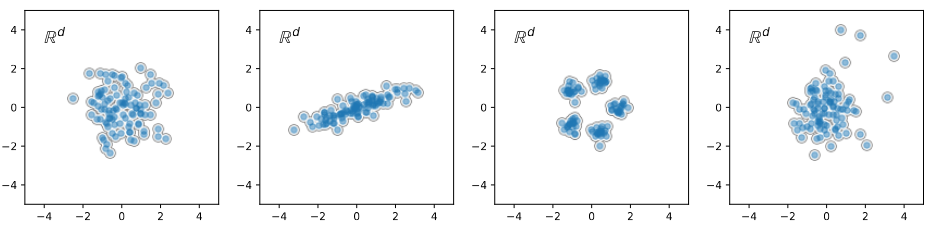
\includegraphics[scale=0.4]{disp}
\end{center}

\subsection{Lagrange multipliers}
The method of Lagrange multipliers is a general framework for finding solutions of constrained optimization problems of the type
\begin{equation*}
	\arg\max_\theta f(\theta) \qquad\qquad g(\theta)=0
\end{equation*}
It consists in the following steps:
\begin{enumerate}
	\item Construct the \textbf{Lagrangian}
	\begin{equation}
		\mathcal{L}(\theta, \lambda) = f(\theta) + \lambda \cdot g(\theta)
	\end{equation}
	where $\epsilon$ is the \textbf{Lagrangian multiplier}
	\item Solve the equation
	\begin{equation}
		\bigtriangledown\mathcal{L}(\theta, \lambda)=0
	\end{equation}
	This includes that the gradient of objective and constraint are aligned but point in opposite direction:
	\begin{equation}
		\bigtriangledown f(\theta) = -\lambda\bigtriangledown g(\theta)
	\end{equation}
\end{enumerate}

\subsection{PCA}
Principal Component Analysis is a specific type of dispersion which can be described in terms of \textbf{directions} in input space.\\
\begin{wrapfigure}[10]{r}{4cm}
	\vspace{-0.5cm}
	\begin{center}
		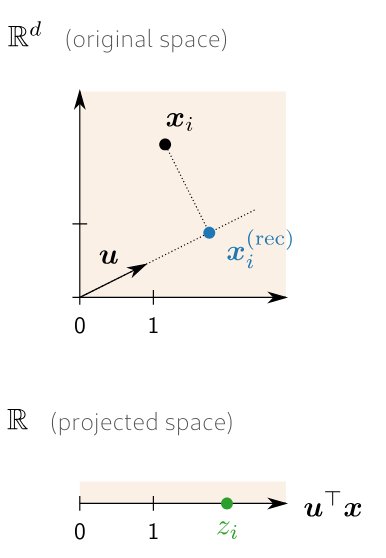
\includegraphics[width=4cm]{pca1}
	\end{center}
\end{wrapfigure}
We start with the following \textbf{preliminaries}:
\begin{itemize}
	\item Let $\mathbf{x}_1, \ldots, \mathbf{x}_N \in \mathbb{R}^d$ be a \textbf{dataset}, where $d$ is the number of \textbf{input features} and $N$ is the number of \textbf{data points}
	\item Let $u \in \mathbb{R}^d$ be a vector of same dimensions, that represents some \textbf{directions} in the input space and is constrained to be of norm $\lvert\lvert u \rvert\rvert = 1$
	\item Data points can be \textbf{projected} onto the direction via the dot product
	\begin{equation}
		\forall_{i=1}^N : z_i = \mathbf{u}^T \mathbf{x}_i
	\end{equation}
	\item The projections can be \textbf{backprojected} on the input space by doing the dot product once again
	\begin{equation}
		\forall_{i=1}^N: \mathbf{x}_i^{\text{(rec)}} = \mathbf{u}\mathbf{u}^T \mathbf{x}_i
	\end{equation}
\end{itemize}
\subsubsection{Formulations}
We have two possible formulations:
\paragraph{Dispersion maximization} Find a projection $z = \mathbf{u}^T \mathbf{x}$ of the data under which the dispersion (variance) is maximized.\\
This means finding a direction $\mathbf{u}$ (with $\lvert\lvert \mathbf{u} \rvert\rvert = 1$) so that the data projected onto this direction $z_1, \ldots, z_N$ has maximum variance.
\begin{equation}
	\arg\max_\mathbf{u} \big[\frac{1}{N} \sum_{i=1}^N(\mathbf{u}^T\mathbf{x}_i-\tilde{m})^2\big] \qquad\qquad \mathbf{u}^T\mathbf{x}_i = z_i
\end{equation}
where $\tilde{m} = \frac{1}{N} \sum_{i=1}^Nz_i$ is the dataset mean in the projected space. \underline{Since we center the data}, we then have $\tilde{m}=0$ and therefore
\begin{equation}
	\label{eq:dispmax}
	\arg\max_\mathbf{u} \big[\frac{1}{N} \sum_{i=1}^N(\mathbf{u}^T\mathbf{x}_i)^2\big]
\end{equation}
\paragraph{Error minimization} Find the direction that minimizes the reconstruction error (MSE) between the original data point $\mathbf{x}$ and its backprojection $\mathbf{x}^{\text{(rec)}} = \mathbf{u}\mathbf{u}^T\mathbf{x}$.\\
This means finding the direction $\mathbf{u}$ (with $\lvert\lvert \mathbf{u} \rvert\rvert = 1$) so that the data projected on the corresponding subspace best reconstructs the original data, having \textbf{minimal squared distance} to it.
\begin{equation}
	\arg\min_\mathbf{u}\big[\frac{1}{N}\sum_{i=1}^N \lvert\lvert \mathbf{x}_i - \mathbf{u}\mathbf{u}^T\mathbf{x}_i\rvert\rvert^2\big] \qquad\qquad \mathbf{u}\mathbf{u}^T\mathbf{x}_i = \mathbf{x}_i^{\text{(rec)}}
\end{equation}

\begin{observation}
	As of Pearson 1901, the two views coincide:
	\begin{align*}
		& \arg\min_\mathbf{u}\big[\frac{1}{N}\sum_{i=1}^N \lvert\lvert \mathbf{x}_i - \mathbf{u}\mathbf{u}^T\mathbf{x}_i\rvert\rvert^2\big]\\
		& = \arg\min_\mathbf{u}\big[\frac{1}{N}\sum_{i=1}^N (\mathbf{x}_i - \mathbf{u}\mathbf{u}^T\mathbf{x}_i)^T(\mathbf{x}_i - \mathbf{u}\mathbf{u}^T\mathbf{x}_i)\big] \\
		& = \arg\min_\mathbf{u}\big[\frac{1}{N}\sum_{i=1}^N \mathbf{x}_i^T\mathbf{x}_i - 2\mathbf{x}_i^T\mathbf{u}\mathbf{u}^T\mathbf{x}_i+(\mathbf{u}\mathbf{u}^T\mathbf{x}_i)^T(\mathbf{u}\mathbf{u}^T\mathbf{x}_i)\big] \\
		& = \arg\min_\mathbf{u}\big[\frac{1}{N}\sum_{i=1}^N -2(\mathbf{x}_i^T\mathbf{u})^2+\mathbf{x}_i^T\mathbf{u}\mathbf{u}^T\mathbf{u}\mathbf{u}^T\mathbf{x}_i\big] \\
		& = \arg\min_\mathbf{u}\big[\frac{1}{N}\sum_{i=1}^N -2(\mathbf{x}_i^T\mathbf{u})^2+(\mathbf{x}_i^T\mathbf{u})^2\big]\\
		& = \arg\max_\mathbf{u} \big[\frac{1}{N} \sum_{i=1}^N(\mathbf{u}^T\mathbf{x}_i)^2\big]
	\end{align*}
	\begin{figure}[!h]
		\hfill
		\subfigure[Error minimization]{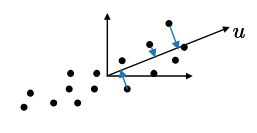
\includegraphics[scale=0.3]{pcamin}}
		\hfill
		\subfigure[Dispersion maximization]{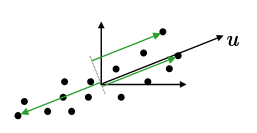
\includegraphics[scale=0.3]{pcamax}}
		\hfill
	\end{figure}
\end{observation}
\subsubsection{Solution}
To find the principal component, we start from the dispersion maximization equation \ref{eq:dispmax} and rewrite it as
\begin{align*}
	& \arg\max_\mathbf{u} \big[\frac{1}{N} \sum_{i=1}^N(\mathbf{u}^T\mathbf{x}_i)^2\big] \\
	& = \arg\max_\mathbf{u} \big[\frac{1}{N} \sum_{i=1}^N (\mathbf{u}^T\mathbf{x}_i)(\mathbf{x}_i^T\mathbf{u})\big]\\
	& = \arg\max_\mathbf{u} \big[\mathbf{u}^T \big(\frac{1}{N} \sum_{i=1}^N\mathbf{x}_i\mathbf{x}_i^T\big)\mathbf{u}\big] \qquad\qquad \lvert\lvert u \rvert\rvert = 1
\end{align*}
where $\Sigma = \frac{1}{N} \sum_{i=1}^N\mathbf{x}_i\mathbf{x}_i^T$ is the \textbf{covariance matrix} that, since it does not depend on $\mathbf{u}$, can be precomputed. We apply the Lagrangian multipliers method:
\begin{enumerate}
	\item We rewrite the constraint as $\lvert\lvert u \rvert\rvert^2 = 1$ and build the Lagrangian
	\begin{equation*}
		\mathcal{L}(\mathbf{u}, \lambda) = \mathbf{u}^T \Sigma\mathbf{u} + \lambda \cdot (1-\lvert\lvert \mathbf{u} \rvert\rvert ^2)
	\end{equation*}
	\item We set the gradient to zero
	\begin{align*}
		& \nabla_\mathbf{u}\mathcal{L}(\mathbf{u}, \lambda)=0 \Rightarrow \Sigma\mathbf{u}=\lambda\mathbf{u} \\
		& \nabla_\lambda\mathcal{L}(\mathbf{u}, \lambda)=0 \Rightarrow \lvert\lvert \mathbf{u}\rvert\rvert^2=1
	\end{align*}
	This means that the solution is an \textbf{eigenvector} of $\Sigma$, in particular
	\begin{align*}
		& \Sigma\mathbf{u}=\lambda\mathbf{u}  \\
		& \mathbf{u}^T\Sigma\mathbf{u}=\lambda\mathbf{u}\mathbf{u}^T \\
		 & \mathbf{u}^T\Sigma\mathbf{u}=\lambda\\
	\end{align*}
	meaning that for the \textit{objective} (left part of the equation) to be maximized, we have to choose the eigenvector in a way that the corresponding eigenvalue $\lambda$ is maximum, therefore the \textbf{leading eigenvector}.
\end{enumerate}
\subsubsection{Problems} The major problems are:
\begin{itemize}
	\item PCA is not very robust to \textbf{outliers}. We need to clean the data before.
	\item PCA does not describe well the data when it's strongly \textbf{non-Gaussian}. It fails to account for the fact that data may vary locally in different directions.
\end{itemize}
\newpage
\subsubsection{Multiple components}
The basic PCA method consists of rewriting the data as the sum of two components: what PCA is able to \textbf{reconstruct} and a \textbf{residue} of what cannot be captured.
\begin{equation}
	\mathbf{x}=\mathbf{u}\mathbf{u}^T\mathbf{x}+(\mathbf{x}-\mathbf{u}\mathbf{u}^T\mathbf{x})
\end{equation}
It's possible to find secondary principal components in the residue with the following algorithm:
\begin{lstlisting}[mathescape=true]
	$X_{\text{res}} \leftarrow X$
	for j=1 to h do
		$w_j \leftarrow \text{PCA}(X_{\text{res}})$
		$X_{\text{res}} \leftarrow X_{\text{res}} -\mathbf{w}_j \mathbf{w}_j^TX_{\text{res}}$
	end for 
\end{lstlisting}
This gives as output a collection of directions $w_1, \ldots, w_h$ which are called the \textbf{principal components}.

\begin{observation}
	The principal components are equivalent to the eigenvectors $\mathbf{u}_1, \ldots, \mathbf{u}_h$ of the covariance matrix $\Sigma$ sorted by decreasing associated eigenvalues $\lambda_1 > \lambda_2 > \ldots > \lambda_h$.\\
	It's therefore sufficient to compute all eigenvectors and eigenvalues of $\Sigma$ and then sort them to get the full solution of PCA.
\end{observation}

\subsubsection{Biplot}
The biplot is a common visualization on the two leading principal components. Each instance corresponds to a point in a scatter plot and its coordinates are given by the pair
\begin{equation*}
	(\mathbf{u}_1^T\mathbf{x}, \mathbf{u}_2^T\mathbf{x})
\end{equation*}
Input features can also be visualized in this plot by projecting their associate canonical coordinate vector in PCA space. They are usually depicted as arrows with the feature name and rescaled for visualization purposes.
\begin{center}
	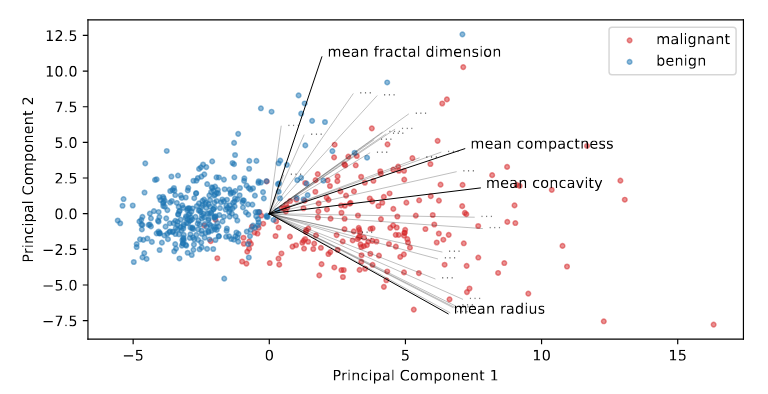
\includegraphics[scale=0.4]{biplot}
\end{center}

\subsubsection{Explained variance}
The \textbf{dispersion} of a multivariate set can be measured as the generalized variance, which can be expressed in therms of $\Sigma$:
\begin{equation}
	s_{\text{tot}}=\mathbb{E}[\lvert\lvert \mathbf{x} - \mathbf{m}\rvert\rvert^2] = \sum_{j=1}^{d} \mathbb{E}[(x_{ij}-m_j)^2] = \text{Tr}(\Sigma)
\end{equation}
where $\mathbb{E}[\cdot]$ denotes an average over points in the dataset.\\
The variation of the data projected on the $k$th principal component can be expressed as
\begin{equation}
	s_k = \mathbb{E}[(\mathbf{u}_k^T(\mathbf{x}-\mathbf{m}))^2] = \mathbf{u}_k^T\Sigma\mathbf{u}_k=\lambda_k
\end{equation}
meaning that it corresponds to the $k$th eigenvalue of the covariance matrix. Therefore the following is true:
\begin{equation}
	\text{Tr}(\Sigma) = \sum_{k=1}^{h}\lambda_k
\end{equation}
This means that PCA produces an additive \textbf{decomposition} of the total dispersion in terms of principal components.
\begin{center}
	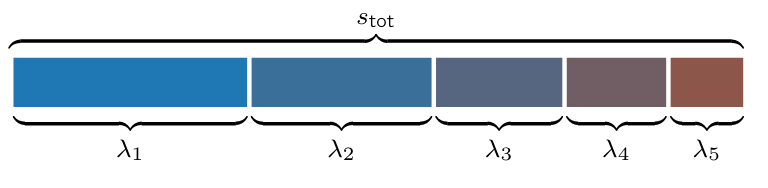
\includegraphics[scale=0.4]{pcadecomp}
\end{center}

\begin{example}
	We could have three two dimensional datasets that have the same overall dispersion $s_\text{tot}$ but distributed differently over principal components:
	\begin{center}
		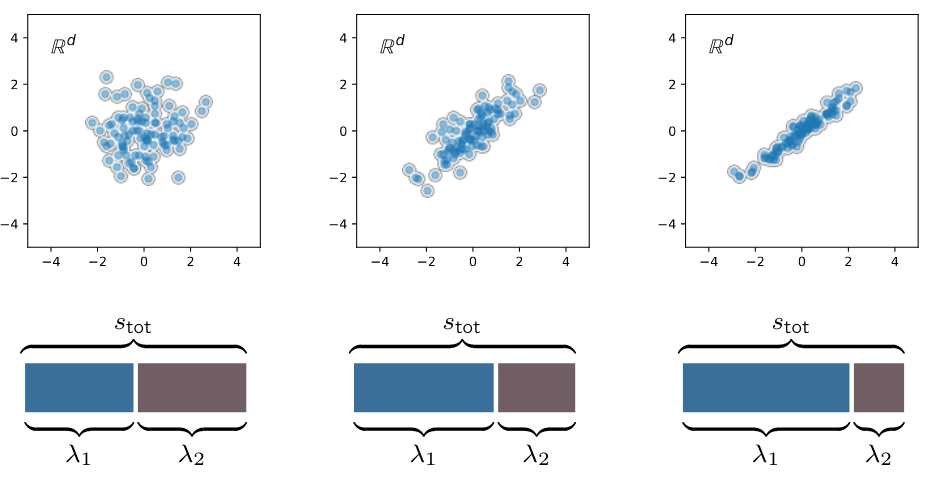
\includegraphics[scale=0.4]{pcaex}
	\end{center}
\end{example}

\subsubsection{Scree plot}
The scree plot is useful to get a picture of the effective \textbf{dimensionality of the data}. If only the first few bars are large, it means that the effective dimensionality is small and the data is simple.
\begin{center}
	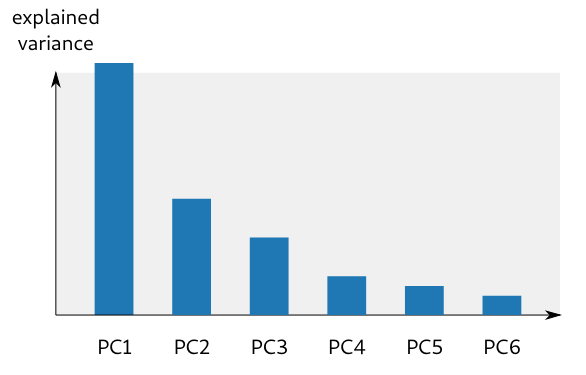
\includegraphics[scale=0.4]{scree}
\end{center}
In this plot, each bar corresponds to the \textit{explained variance} associated to a particular principal component. Its height is given by the associated \textit{eigenvalue}. It can be interpreted as the share of the total variance explained by this component.
\begin{note}
	Sometimes the information is better depicted as a \textbf{cumulative plot} where the $k$th bar indicates the variance obtained retaining the leading $k$ principal components.
\end{note}

\subsubsection{Applications}
PCA is not used only to describe the data but also to remove certain factors that contribute to data dispersion, such as:
\begin{itemize}
	\item \textbf{Artifact} removal: it may be reasonable to remove first principal components (e.g. eye blinking in EEG)
	\item \textbf{Denoising}: remove last principal components
\end{itemize}
\subsubsection{Improvements}
Since many data are high-dimensional, the standard implementation of the PCA would have to compute a covariance matrix $\Sigma$ of $d \times d$ size, which would be time and space consuming.
\paragraph{SVD}
\begin{definition}[SVD]
	A singular value decomposition factorizes a matrix $M = U \Lambda V$ where
	\begin{itemize}
		\item $U$ contains the eigenvectors of $MM^T$
		\item $V$ contains the eigenvectors of $M^TM$
		\item $\Lambda$ is a diagonal matrix, with diagonal elements of $\Lambda^2$ containing the eigenvalues of $MM^T$
	\end{itemize}
\end{definition}
Since SVD extracts the eigenvectors and eigenvalues of the matrix $MM^T$ and PCA solutions corresponds to those of the covariance matrix $\Sigma$, we can compute the latter by setting $\Sigma = MM^T$, therefore
\begin{equation}
	M = \frac{1}{\sqrt{N}}X
\end{equation}
The \textbf{algorithm} is the following:
\begin{enumerate}
	\item Let $X$ be our data matrix of size $d \times N$
	\item Define $M = \frac{1}{\sqrt{N}}X$
	\item Feed the matrix $M$ to SVD and get $U$, $\Lambda$ and $V$
	\item PCA eigenvectors are the columns of $U$ while eigenvalues are the diagonal elements of $\Lambda^2$
\end{enumerate}
When computing the matrix $U$ we have the option to not calculate all the matrices, which for $d>N$ would be a huge amount. In that case $U$ is $d \times N$.\\
The \textbf{complexity} of the algorithm is $O(\min(N^2d,d^2N))$, but when $d \approx N$, it becomes as bad as the one for computing the eigenvectors of $\Sigma$ ($O(d^3)$).

\paragraph{Power Iteration} Since in large datasets even SVD is prohibitive and often we just need the first principal components, we can use the power iteration algorithm to get them. The following finds the \textbf{first} principal component:
\begin{lstlisting}[mathescape=true]
	$u \approx$ random()
	repeat
		$v \leftarrow \Sigma \mathbf{u}$
		$\mathbf{u} \leftarrow \frac{\mathbf{v}}{\lvert\lvert \mathbf{v} \rvert\rvert}$
	until convergence
\end{lstlisting}
It \textbf{always} converges \textbf{exponentially fast}.\\
To get the following ones:
\begin{lstlisting}[mathescape=true]
	$\Sigma = \frac{1}{N}XX^T$
	for j=1 to h do
		$\mathbf{u}_j \leftarrow \text{POWIT}(\Sigma)$
		$\Sigma \leftarrow \Sigma - \mathbf{u}_j \mathbf{u}_j^T\Sigma$
	end for
\end{lstlisting}